\tikzstyle{wired}=[draw=gray!30, line width=0.15mm]
\tikzstyle{number}=[anchor=center, color=white]

% Sectors are numbered 0-19 counterclockwise from the top.

% \strip{color}{sector}{outer_radius}{inner_radius}
\newcommand{\strip}[4]{
    \filldraw[#1, wired]
      ({18 *  #2}      :                   #3) arc
      ({18 *  #2}      : {18 * (#2 + 1)} : #3) --
      ({18 * (#2 + 1)} :                   #4) arc
      ({18 * (#2 + 1)} : {18 *  #2}      : #4) -- cycle;
}

% \sector{color}{sector}{radius}
\newcommand{\sector}[3]{
    \filldraw[#1, wired]
      (0, 0) --
      ({18 * #2} :                   #3) arc
      ({18 * #2} : {18 * (#2 + 1)} : #3) -- cycle;
}

% 81 degrees = 4.5 sectors.
% The rotation leaves 20 at the top.
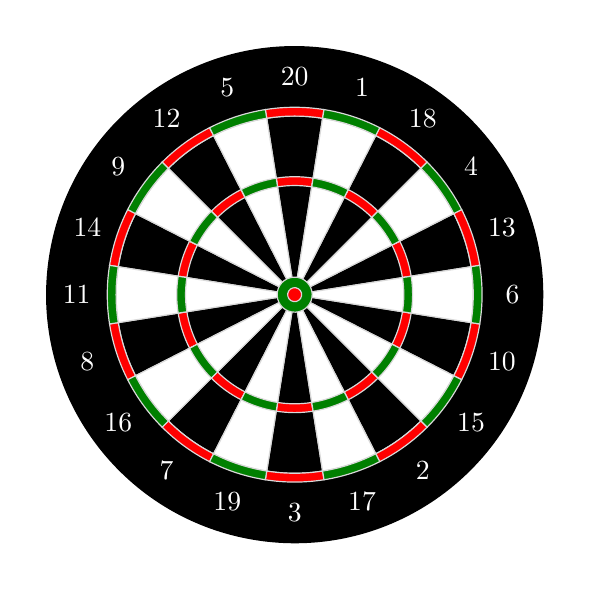
\begin{tikzpicture}[rotate=81, scale=.14]

  % These are the official dartboard dimensions as per BDO's regulations.

  % The whole board's background.
  \fill[black] (0, 0) circle (225.5mm);

  % Even sections.
  \foreach\i in {0,2,...,18} {
    \sector{black}{\i}{162mm}
    \strip{Red}{\i}{170mm}{162mm} % Double strip.
    \strip{Red}{\i}{107mm}{ 99mm} % Treble strip.
  }

  % Odd sections.
  \foreach\i in {1,3,...,19} {
    \sector{white}{\i}{162mm}
    \strip{Green}{\i}{170mm}{162mm} % Double strip.
    \strip{Green}{\i}{107mm}{ 99mm} % Treble strip.
  }

  % Bull's ring and eye.
  \filldraw[Green, wired] (0, 0) circle (15.9mm);
  \filldraw[Red,   wired] (0, 0) circle (6.35mm);

  % Labels.
  \foreach \sector/\label in {%
      0/20,  1/ 1,  2/18,  3/ 4,  4/13,
      5/ 6,  6/10,  7/15,  8/ 2,  9/17,
     10/ 3, 11/19, 12/ 7, 13/16, 14/ 8,
     15/11, 16/14, 17/ 9, 18/12, 19/ 5}%
  {
    \node[number] at ({18 * (-\sector + .5)} : 197.75mm) {\label};
  }

\end{tikzpicture}

